% Author: Till Tantau
% Source: The PGF/TikZ manual

\documentclass{article}

\usepackage{pgf}
\usepackage{tikz}
\usepackage{varwidth}
\usetikzlibrary{arrows,automata}
\usepackage[latin1]{inputenc}
\usetikzlibrary{arrows,automata}
\usetikzlibrary{positioning}


\tikzset{
    state/.style={
           rectangle,
           rounded corners,
           draw=black, very thick,
           minimum height=2em,
           inner sep=2pt,
           text centered,
           },
}
\begin{document}
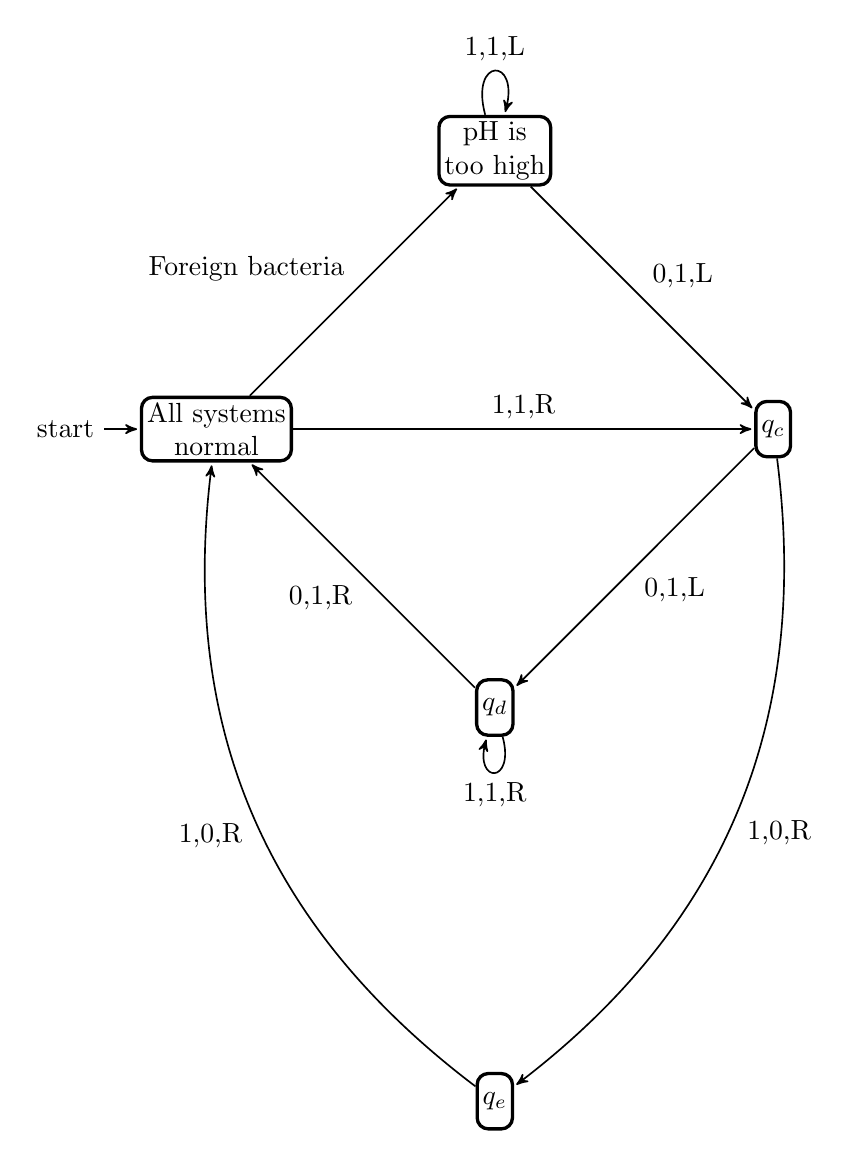
\begin{tikzpicture}[->,>=stealth',shorten >=1pt,auto,node distance=5cm,
                    semithick]
  \tikzstyle{every state}=[fill=gray,draw=none,text=black]

  \node[initial,state,align=center] (A)                    {All systems \\ normal};
  \node[state, align=center]         (B) [above right of=A] {pH is \\ too high};
  \node[state, align=center]         (D) [below right of=A] {$q_d$};
  \node[state, align=center]         (C) [below right of=B] {$q_c$};
  \node[state, align=center]         (E) [below of=D]       {$q_e$};
  %\node (example-varwidth-linebreak) [draw, align=center]{\begin{varwidth}{3cm}This is a demonstration \\ text for showing how line breaking works.\end{varwidth}};


  \path (A) edge              node {Foreign bacteria} (B)
            edge              node {1,1,R} (C)
        (B) edge [loop above] node {1,1,L} (B)
            edge              node {0,1,L} (C)
        (C) edge              node {0,1,L} (D)
            edge [bend left]  node {1,0,R} (E)
        (D) edge [loop below] node {1,1,R} (D)
            edge              node {0,1,R} (A)
        (E) edge [bend left]  node {1,0,R} (A);
\end{tikzpicture}

\end{document}
